\documentclass[letterpaper,12pt]{article}
\usepackage{tabularx} % extra features for tabular environment
\usepackage{amsmath}  % improve math presentation
\usepackage{float}
\usepackage{pdfpages}


\usepackage{graphicx} % takes care of graphic including machinery
\graphicspath{ {./figures/} }
%\usepackage[margin=1in,letterpaper]{geometry} % decreases margins
%\usepackage{cite} % takes care of citations
\usepackage[final]{hyperref} % adds hyper links inside the generated pdf file
\hypersetup{
	colorlinks=true,       % false: boxed links; true: colored links
	linkcolor=blue,        % color of internal links
	citecolor=blue,        % color of links to bibliography
	filecolor=magenta,     % color of file links
	urlcolor =blue         
}
\usepackage[margin = 1in,headsep=0.5cm,headheight=2cm,letterpaper]{geometry} 

\usepackage{fancyhdr}
\pagestyle{fancy}
\lhead{Student 1 : Ahmet Akman 2442366 \\ Student 2: Yusuf Toprak Yıldıran 2444149 \\ Assistant: Onur Selim Kılıç}
\rhead{Date: \today \\ Group: Wednesday Morning - 5} 
%\cfoot{center of the footer!}
\renewcommand{\headrulewidth}{0.1pt}
%

%\renewcommand{\footrulewidth}{0.4pt}



\begin{document}
\thispagestyle{empty}

\title{Spring 2022 EE214 Experiment 2  \protect\\ Miscellaneous Op-Amp Circuits}
\author{Ahmet Akman 2442366 \protect\\ Yusuf Toprak Yıldıran 2444149 \protect\\ Assistant: Onur Selim Kılıç}
\date{\today}
\maketitle
\tableofcontents
%\begin{abstract}
%abstract
%\end{abstract}
\section{Introduction}
In this experiment, miscellaneous op-amp circuits, three different setups of op-amp circuity are investigated. First, an independent current source circuit is set and its behavior is required to be characterized. Then the clipper circuit is constructed, and the output is needed to be observed. Lastly, a negative resistance converter with two zener is built with two different setups. First, its i-v characteristics are expected to be observed, then a square wave generator is expected to be set.
\section{Experimental Results and Discussion}
The results of the experiment are discussed in the following steps.
\subsection{Step 1}
In this step independent current source circuit given in Figure 1 is constructed. A potentiometer with 10K\(\Omega\) is connected to the one port as \(R_L\).
\begin{figure}[H]
    \centering
    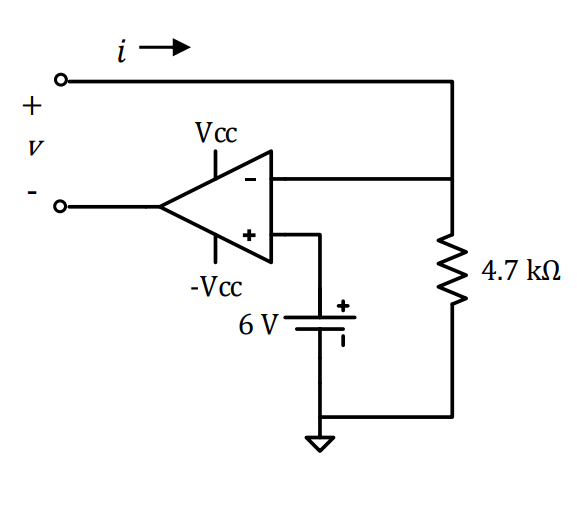
\includegraphics[width = 0.75\textwidth]{1SCH.png}
    \caption{Circuit schematic for the step 1}
\end{figure} 
To be able to obtain the maximum value of the resistance in which the one port still functions as a independent current source, the potentiometer is meticulously adjusted. So , the parameters given in Figure 1 is obtained.
\begin{table}[H]
    \begin{center}
        \caption{Resistance reading by color code convention.}
        \vspace{2mm}
        \begin{tabular}{||c | c ||} 
            \hline
            The Current Value & Corresponding Resistance \\ [0.5ex] 
            \hline\hline
            1.24 mA & 8k\(\Omega\)    \\
            \hline
        \end{tabular}
    \end{center}
\end{table}

\subsection{Step 2}
In this step the 

\begin{figure}[H]
    \centering
    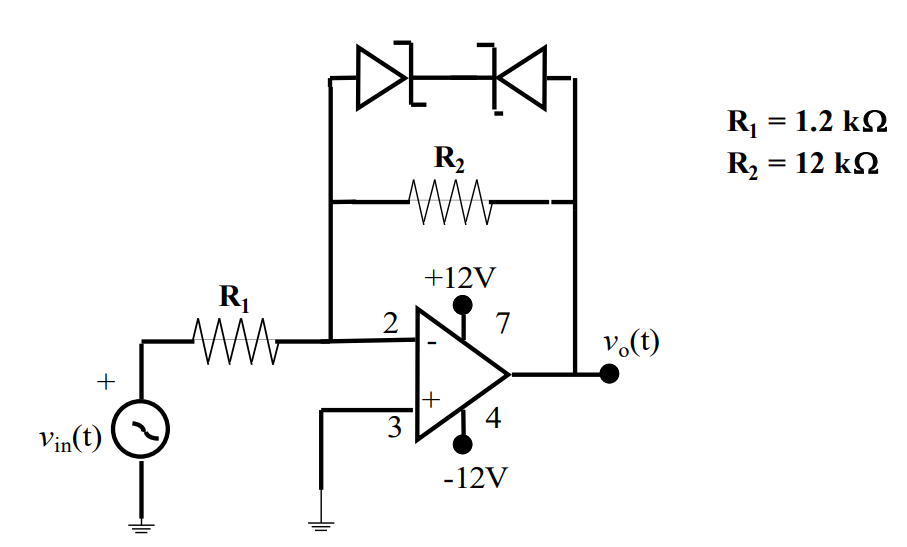
\includegraphics[width = 0.75\textwidth]{2SCH.png}
    \caption{Circuit schematic for the step 2}
\end{figure} 

\subsection{Step 3}


\begin{figure}[H]
    \centering
    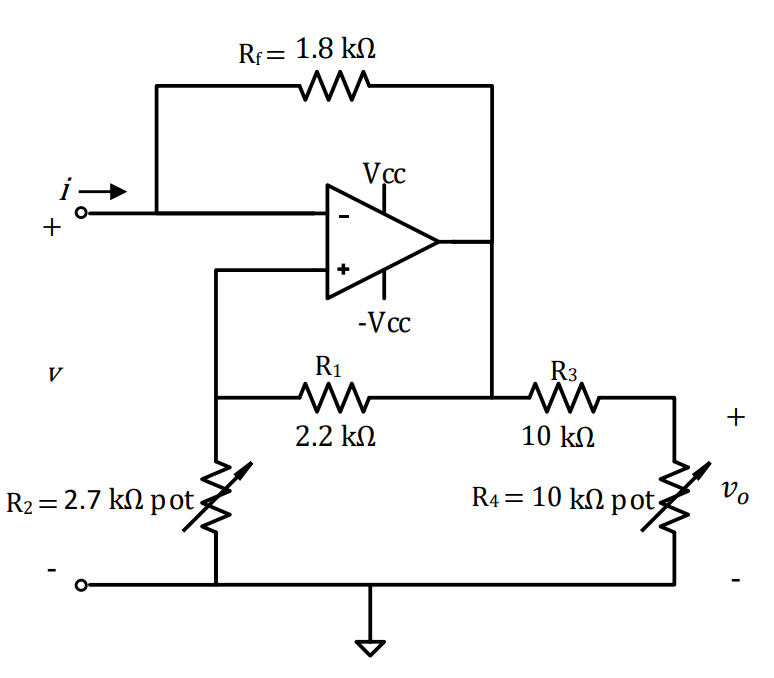
\includegraphics[width = 0.75\textwidth]{3SCH.png}
    \caption{Circuit schematic for the step 3}
\end{figure} 

\subsubsection{a)}

\subsubsection{b)}

\section{Conclusion}

helll
rfgtgtgtgt
\section*{Appendix A}
\begin{itemize}
    \item PreLab Preparation 4 hours
    \item Experimental Work 2  hours
    \item Report Writing 4 hours
\end{itemize}

\end{document}

%%%%%%%%%%%%%%%%%%%%%%   EXAMPLE TABLE   %%%%%%%%%%%%%%%%%%%%%%%%%%%%%%%%
\begin{table}[H]
\begin{center}
    \caption{Resistance reading by color code convention.}
    \vspace{2mm}
    \begin{tabular}{||c | c | c||} 
        \hline
        Color Order & Value & Tolerance \\ [0.5ex] 
        \hline\hline
        Brown / Black / Red / Gold & 1k\( \Omega \) & \( \% \) 5  \\ 
        \hline
        Yellow / Violet / Red / Gold & 4.7k\( \Omega \) & \( \% \) 5   \\
        \hline
        Brown / Grey / Orange / Gold & 18k\( \Omega \) & \( \% \) 5  \\ [1ex] 
        \hline
    \end{tabular}
\end{center}
\end{table}


%%%%%%%%%%%%%%%%%%%%%%   EXAMPLE IMAGE   %%%%%%%%%%%%%%%%%%%%%%%%%%%%%%%%
\begin{figure}[H]
\centering
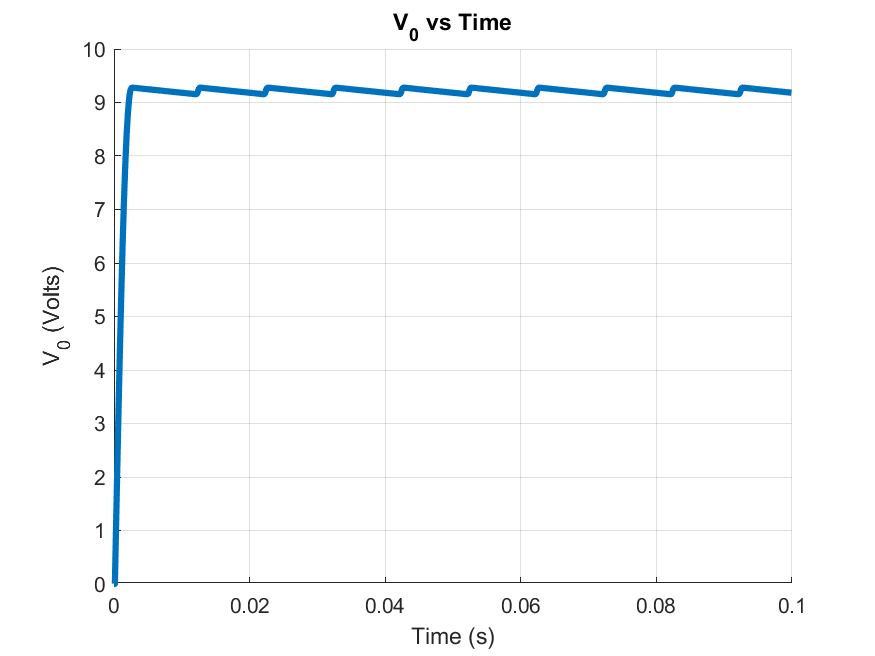
\includegraphics[width = 0.75\textwidth]{5.png}
\caption{Circuit schematic for the step 5}
\end{figure} 

%%%%%%%%%%%%%%%%%%%%%%   EXAMPLE IMAGE FROM PDF   %%%%%%%%%%%%%%%%%%%%%%%%%%%%%%%%
\begin{figure}[H] \centering{
	\includegraphics[scale=0.25]{2a_plot.pdf}}
	\caption{Experiment 2}
\end{figure}
	